\chapter{Background}

In this chapter I am going to introduce the reader to the concepts that are necessary to understand the research presented in this thesis. The chapter is divided into three sections. The first section provides an overview of Variational Autoencoders (VAEs) and their applications. The second section introduces Vector Quantized VAEs (VQ-VAEs). The third section introduces Multitask VAEs (MT-VAEs), which are the main focus of this thesis.

\section{VAEs}

Variational Autoencoders (VAEs), first introduced in 2013 by Kingma and Welling\cite{kingma2022autoencoding}, have become a prominent class of generative models in the field of machine learning.  At their core, VAEs consist of an encoder network with parameters $\phi$ that maps data points $x$ into a latent space $z$ and a decoder network with parameters $\theta$ that generates data $\hat{x}$ from latent representations\cite{Kingma_2019}. 

The key innovation that makes VAEs work is the introduction of a probabilistic interpretation of the latent space. More specifically, VAEs assume that the latent space $z$ is a random variable that follows a certain prior distribution $p(z)$, which is typically a Gaussian distribution and that the mapping from the latent space to the data space is also probabilistic\cite{kingma2022autoencoding}.

The optimization target for VAEs is the evidence lower bound (ELBO) which is: \[ L(\theta, \phi) = \mathbb{E}_{q_{\phi}(z|x)} [\log p_{\theta}(z, x) - \log q_{\phi}(z|x)] \] where $q_{\phi}(z|x)$ is the encoder distribution, $p_{\theta}(z, x)$ is the decoder distribution and $p(z)$ is the prior distribution. The individual datapoint ELBO and its gradient is, in general, intractable. However, this is where reparametrization trick comes which is discussed in the next section.
\subsection{Reparametrization Trick}

A crucial aspect of VAEs is the reparametrization trick, which is introduced to enable the backpropagation of gradients through the sampling operation. In a standard VAE, the encoder network learns to parameterize a distribution in the latent space, which is usually a assumed to be a Gaussian distribution with a mean $\mu$ and a standard deviation $\sigma$. The reparametrization trick involves sampling from a standard Gaussian distribution $\epsilon \sim \mathcal{N}(0,1)$ and then transforming the samples into samples from the learned distribution using the following equation: \[ z = \mu + \sigma \odot \epsilon \] where $\odot$ denotes the element-wise multiplication\cite{kingma2022autoencoding}.This differentiable transformation enables for the stochasticity to be decoupled from the network parameters, allowing for the gradients to flow through the entire network.

The probabilistic nature of VAE's make them not only suitable for generative tasks, but also facilitates the generation of diverse samples. This property makes VAEs particularly useful for tasks such as image synthesis, where it excels at capturing the underlying structure and variability of the data\cite{Kingma_2019}.

\begin{figure}[H]
    \centering
    \makebox[\textwidth]{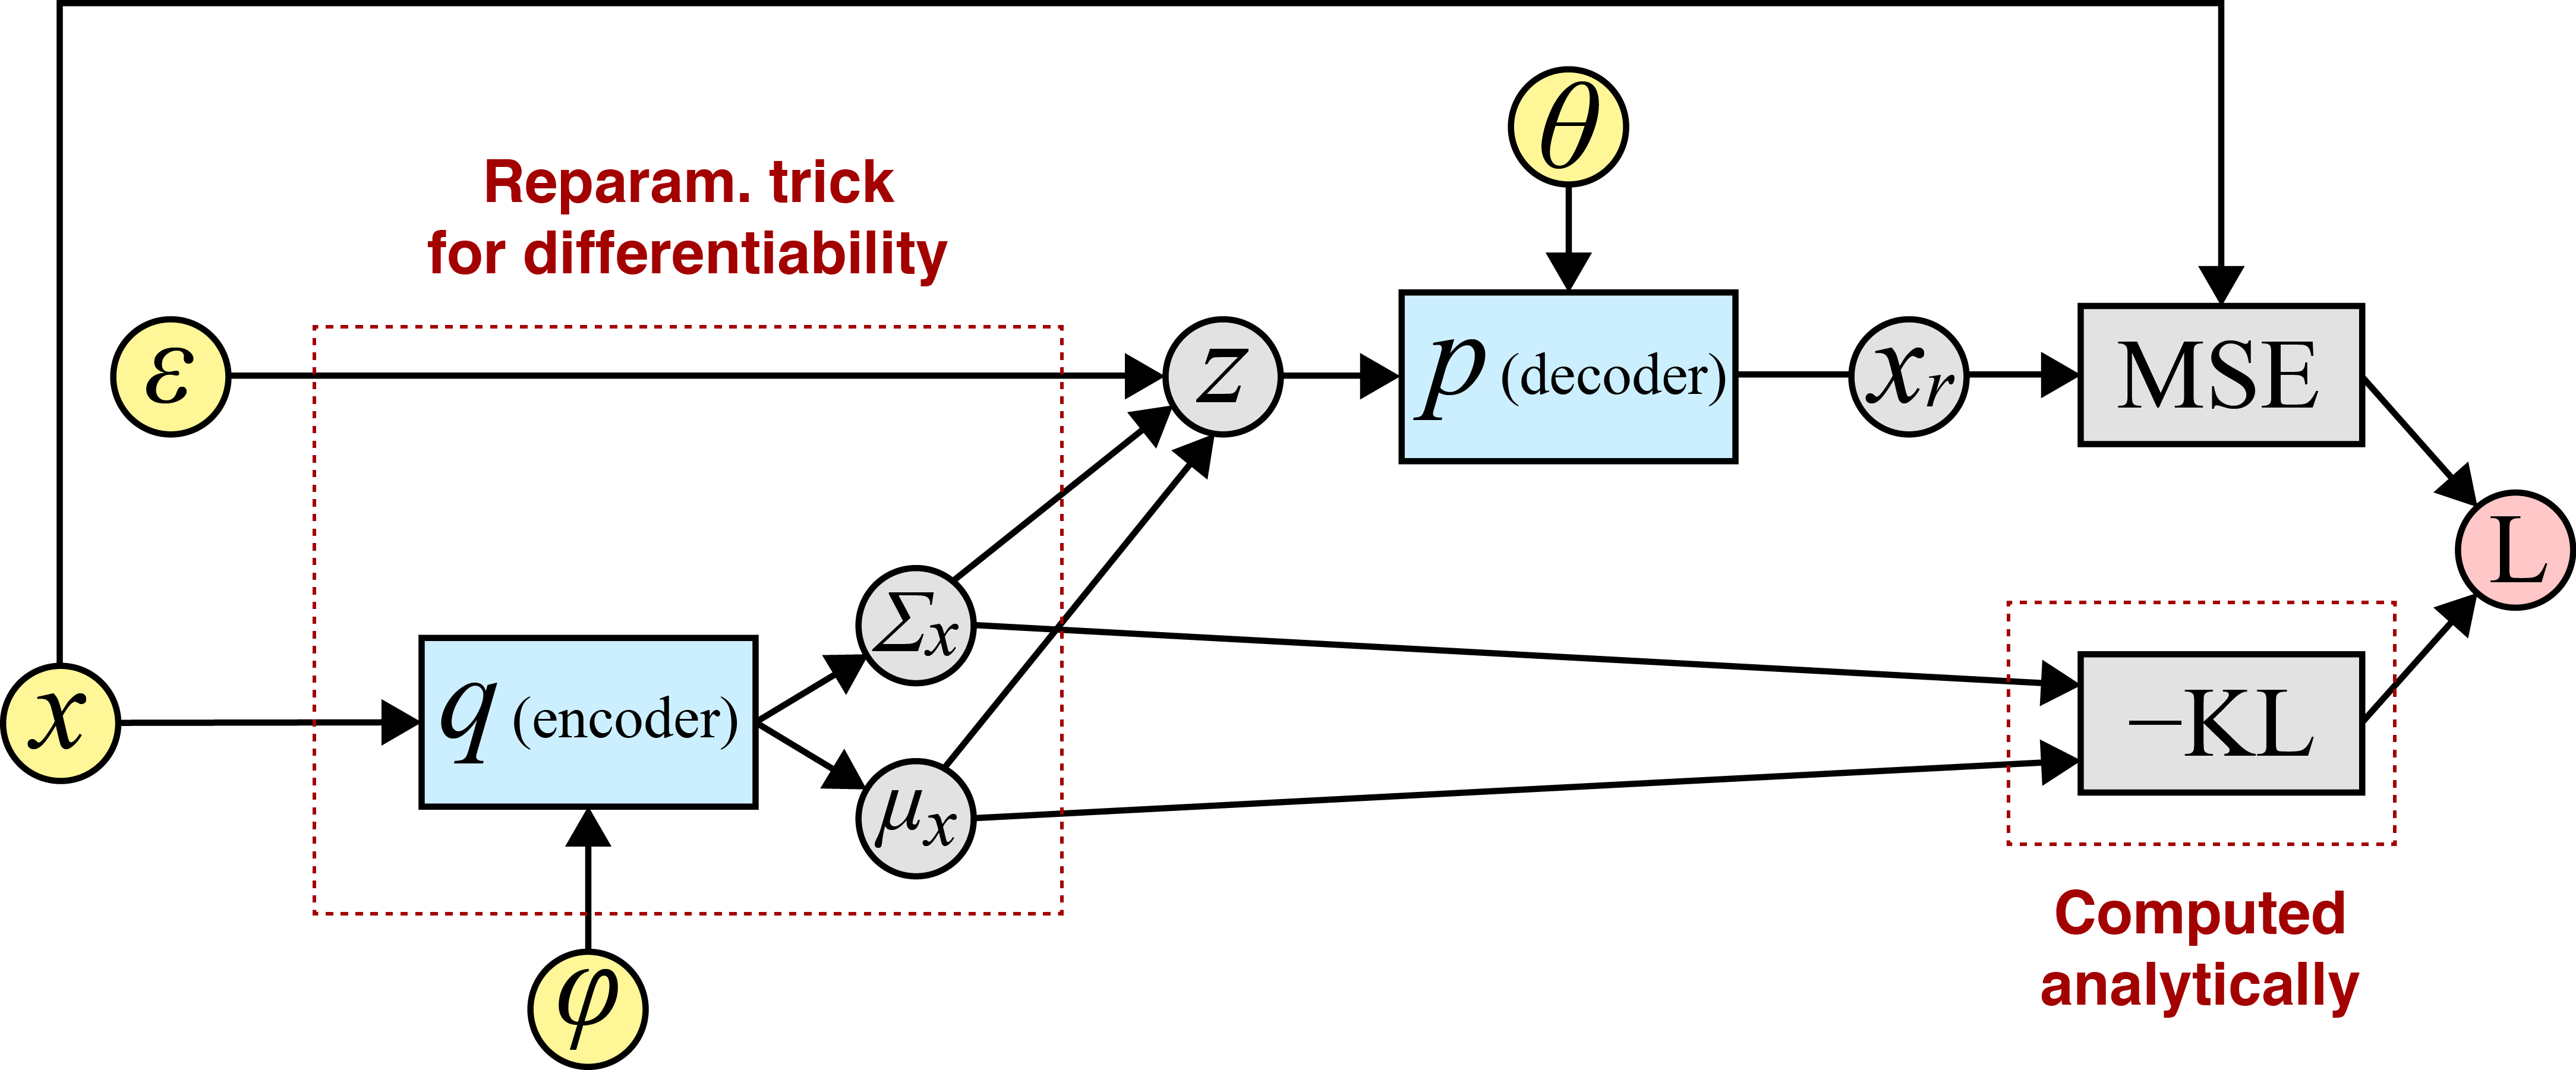
\includegraphics[width=\textwidth]{figures/vae}}

    \caption{ The architecture of VAEs.}
  	\medskip 
	\hspace*{15pt}\hbox{\scriptsize Credit: Aäron van den Oord et al.}
    \label{VAEFigure}

\end{figure}

\section{Vector Quantized VAEs}

Vector Quantized VAEs (VQ-VAEs) are a variant of VAEs that were introduced in 2017 by Aäron van den Oord et al\cite{vqvae}. VQ-VAEs successfully combine the VAE framework with discrete latent representations using a technique called Vector Quantization. 

\begin{figure}[H]
    \centering
    \makebox[\textwidth]{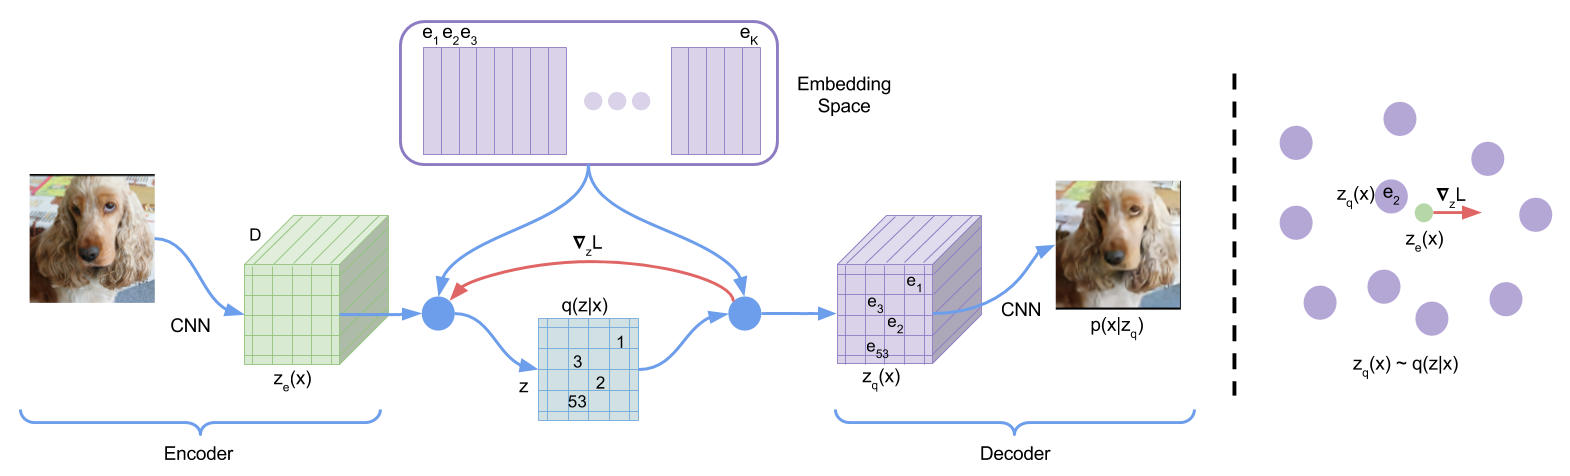
\includegraphics[width=\textwidth]{figures/vq_vae}}

    \caption{On the left side there is a figure describing the VQ-VAE architecture. On the right side there is visualization of the latent space whilst training. The figure is taken from \cite{vqvae}.}
  	\medskip 
	\hspace*{15pt}\hbox{\scriptsize Credit: Aäron van den Oord et al.}
    \label{VQVAEFigure}

\end{figure}
